\documentclass[11pt,a4paper]{article}

\usepackage[utf8]{inputenc}
\usepackage[T1]{fontenc}
\usepackage{mathptmx}
\usepackage{tgtermes}
\usepackage[french]{babel}
\frenchsetup{StandardItemLabels=true,AutoSpacePunctuation=false,SmallCapsFigTabCaptions=false}
\addto\captionsfrench{\renewcommand{\tablename}{Tableau}\renewcommand{\figurename}{Figure}}
\usepackage[a4paper,margin=2cm]{geometry}
\usepackage{microtype}
\usepackage{graphicx}
\usepackage{booktabs}
\usepackage{array}
\usepackage{tabularx}
\usepackage{caption}
\usepackage{enumitem}
\usepackage{titlesec}
\usepackage[hidelinks]{hyperref}

\DeclareCaptionLabelSeparator{deuxpoints}{~:\ }
\captionsetup{font=small,labelfont=bf,labelsep=deuxpoints,skip=6pt}
\captionsetup[table]{position=top}

\setlength{\parindent}{0pt}
\setlength{\parskip}{0.45em}
\setlist[itemize]{topsep=0pt,partopsep=0pt,itemsep=3pt,parsep=0pt}
\renewcommand{\topfraction}{0.85}
\renewcommand{\bottomfraction}{0.6}
\renewcommand{\textfraction}{0.1}
\renewcommand{\floatpagefraction}{0.8}
\setlength{\textfloatsep}{12pt plus 2pt minus 4pt}
\titleformat{\section}{\large\bfseries}{\thesection.}{0.5em}{}
\titleformat{\subsection}{\normalsize\bfseries}{\thesubsection}{0.6em}{}
\titlespacing*{\section}{0pt}{1.4em}{0.4em}
\titlespacing*{\subsection}{0pt}{1.1em}{0.3em}
\titleformat{\subsubsection}{\normalsize\itshape\bfseries}{\thesubsubsection}{0.6em}{}
\titlespacing*{\subsubsection}{0pt}{0.9em}{0.25em}
\renewcommand{\arraystretch}{1.15}

\DeclareUnicodeCharacter{03C3}{\ensuremath{\sigma}}
\DeclareUnicodeCharacter{03A3}{\ensuremath{\Sigma}}
\DeclareUnicodeCharacter{03B7}{\ensuremath{\eta}}
\DeclareUnicodeCharacter{221A}{\ensuremath{\surd}}
\DeclareUnicodeCharacter{221D}{\ensuremath{\propto}}
\DeclareUnicodeCharacter{2192}{\ensuremath{\rightarrow}}
\DeclareUnicodeCharacter{2248}{\ensuremath{\approx}}
\DeclareUnicodeCharacter{207A}{\ensuremath{^{+}}}
\DeclareUnicodeCharacter{207B}{\ensuremath{^{-}}}
\DeclareUnicodeCharacter{2070}{\ensuremath{^{0}}}
\DeclareUnicodeCharacter{00B3}{\ensuremath{^{3}}}
\DeclareUnicodeCharacter{2074}{\ensuremath{^{4}}}
\DeclareUnicodeCharacter{2075}{\ensuremath{^{5}}}
\DeclareUnicodeCharacter{2077}{\ensuremath{^{7}}}

\begin{document}

\begin{center}
{\LARGE\bfseries TP2 - Plongements de mots statiques\par}
\vspace{0.4em}
{\large Modèles de langage - M2 Informatique IAAA, Aix-Marseille Université\par}
\vspace{0.6em}
{Leader : Léandre Raeth \qquad Follower : Sarah Boshra\par}
\vspace{0.3em}
{Novembre 2026\par}
\end{center}
\vspace{0.5em}

\section{Introduction}

L’objectif de ce projet est, dans un premier temps, de programmer un modèle de plongements (embeddings) de mots statiques inspiré de word2vec, plus précisément de la méthode skip-gram avec échantillonnage négatif.

Un plongement associe à chaque mot un vecteur qui représente les contextes dans lesquels il apparaît, pour que deux mots voisins (vélo, bicyclette) aient des vecteurs proches.

À partir de ce premier travail, nous pouvons explorer deux pistes~:

La première (8.1) cherche à améliorer la qualité des plongements en reprenant des techniques d’un article scientifique et du code officiel word2vec.

Cette piste interroge la différence entre un modèle tel qu’il est décrit dans un article et le modèle tel qu’il est effectivement implémenté. L’intérêt est de chercher à pousser la précision du modèle et de comprendre l’impact de ces améliorations.

La deuxième (8.2) teste si l’arithmétique des vecteurs encode du sens. C’est-à-dire, est-ce que des opérations mathématiques entre vecteurs sont vérifiées~: roi - homme + femme ≈ reine. Elle vérifie cette affirmation célèbre et à quel point elle peut être étendue, sur quels types de relations elle tient, et les différentes manières de chercher efficacement le mot le plus proche d’un vecteur.

En section 2, nous présentons le modèle initial et sa performance de référence, puis les deux pistes que nous avons creusées (sections 2.1 et 2.2). Nous concluons en section 3.

\section{Modèle Initial}

\subsection*{Le modèle}

Le modèle que nous avons programmé est le skip-gram avec échantillonnage négatif décrit dans le sujet. Il fonctionne via un classifieur binaire qui reçoit deux mots, un mot cible m et un mot c, et estime la probabilité P(+|m,c) que c apparaisse dans le contexte de m.

P(+|m,c) = σ(m·c), avec σ(x) = 1/(1 + e\textasciicircum{}(-x)). La probabilité complémentaire vaut P(-|m,c) = 1 - σ(m·c) = σ(-m·c). Chaque mot possède deux vecteurs distincts. Deux matrices contiennent ces vecteurs~: M contient le vecteur du mot lorsqu’il joue le rôle de mot cible, C celui du mot lorsqu’il joue le rôle de mot de contexte.

À la fin de l’apprentissage, seule la matrice M est conservée comme plongements. (La matrice C n’est qu’un outil de l’optimisation). Pour chaque mot cible m, le mot cpos situé dans une fenêtre de L mots avant et après m donne un exemple positif (m, cpos). À chaque exemple positif sont associés k exemples négatifs (m, cneg), où cneg est un mot tiré uniformément au hasard dans le vocabulaire.

Un exemple positif et ses k négatifs forment un mini-batch, qui est l’unité de mise à jour du modèle.

La fonction de perte est l’opposé du logarithme de la probabilité d’avoir bien classé tous les exemples~: L = -[ log σ(m·cpos) + Σ\_\{i=1..k\} log σ(-m·cneg\_i) ].

Les paramètres sont mis à jour par descente de gradient stochastique, c’est-à-dire après chaque mini-batch, avec un taux d’apprentissage η.

Pour initialiser M et C, nous avons tiré chaque coordonnée uniformément dans l’intervalle [-0,5/n~; 0,5/n], où n est la dimension des plongements, soit des valeurs comprises entre -0,005 et 0,005 pour n = 100.

Ainsi, avec des vecteurs de très petite norme, tous les produits scalaires sont proches de 0, donc toutes les probabilités proches de 0,5.

Les hyperparamètres sont ceux fournis par le sujet~: dimension n = 100, demi-fenêtre L = 2, k = 10 négatifs par positif, taux d’apprentissage η = 0,1, 5 époques, et un mot n’a un plongement que s’il apparaît au moins minc = 5 fois.

\subsection*{Données}

Le sujet indique que les plongements doivent être appris sur le corpus \emph{Le comte de Monte-Cristo}, mais ce corpus ne nous a pas été fourni avec les données. Nous avons donc travaillé sur un autre corpus, \texttt{train\_500k}, partagé au sein de la promotion.

Il s’agit de texte français en minuscules dont la ponctuation est séparée des mots par des espaces, et qui tient sur une seule ligne.

Cette substitution empêche de comparer strictement nos chiffres à celui du sujet.

Nous découpons le texte aux marqueurs de fin de phrase, nous supprimons les symboles qui ne contiennent aucun caractère alphanumérique, et nous écartons les phrases de moins de deux mots, qui ne peuvent produire aucune paire.

Le Tableau 1 donne les caractéristiques du corpus obtenu.

\begin{table}[!htbp]
\centering
\small
\caption{caractéristiques du corpus d’apprentissage après prétraitement.}
\begin{tabular}{lr}
\toprule
\textbf{grandeur} & \textbf{valeur} \\
\midrule
phrases & 21~820 \\
mots (occurrences) & 391~622 \\
vocabulaire (mots d’au moins 5 occurrences) & 6~759 \\
occurrences conservées après filtrage des mots rares & 362~841 (92,7~\%) \\
paires (cible, contexte) pour L = 2 & 1~320~894 \\
\bottomrule
\end{tabular}
\end{table}

Les mots les plus fréquents sont \emph{de} (16~528 occurrences), \emph{la} (10~967), \emph{le} (8~343), \emph{il} (8~076) et \emph{et} (7~156). Cette forte inégalité des fréquences sera importante pour la piste 1.

\subsection*{Protocole d’évaluation}

La qualité des plongements est mesurée sur 100 triplets (m, m⁺, m⁻) fournis avec le sujet. Ils sont construits de sorte que m⁺ soit plus proche de m, par le sens, que m⁻ (par exemple \emph{vélo, bicyclette, chat}). Un triplet est réussi lorsque la similarité cosinus entre m et m⁺ est strictement supérieure à celle entre m et m⁻. Le taux de réussite est la proportion de triplets réussis parmi les triplets évaluables.

Tous les triplets ne le sont pas~: nous obtenons 86 triplets évaluables sur 100.

Certains triplets contiennent au moins un mot absent de notre vocabulaire. Les mots manquants sont caractéristiques du roman (\emph{cachot}, \emph{geôlier}, \emph{armateur}, \emph{marin} ou \emph{bâtiment}), ce qui indique que le fichier d’évaluation a été conçu à partir du corpus Monte-Cristo.

Nos taux de réussite portent donc sur 86 triplets et certains mots testés ont peu d’occurrences dans notre corpus. Cette réserve vaut pour tous les résultats du rapport.

\subsection*{Résultats de référence}

L’apprentissage dépend du hasard (initialisation des matrices, ordre des paires, tirage des négatifs), un entraînement isolé ne permet donc pas de conclure.

Nous avons donc entraîné le modèle 10 fois avec des graines aléatoires différentes (0 à 9), à hyperparamètres identiques, et nous rapportons la moyenne et l’écart-type d’échantillon des 10 taux de réussite. Le Tableau 2 donne les 10 valeurs.

\begin{table}[!htbp]
\centering
\small
\caption{taux de réussite du modèle initial, selon la graine.}
\begin{tabular}{lcccccccccc}
\toprule
\textbf{graine} & \textbf{0} & \textbf{1} & \textbf{2} & \textbf{3} & \textbf{4} & \textbf{5} & \textbf{6} & \textbf{7} & \textbf{8} & \textbf{9} \\
\midrule
taux (\%) & 80,2 & 80,2 & 75,6 & 81,4 & 76,7 & 80,2 & 75,6 & 77,9 & 79,1 & 80,2 \\
\bottomrule
\end{tabular}
\end{table}

Le taux de réussite moyen du modèle initial est de \textbf{78,7~\%}, avec un écart-type de \textbf{2,1 points} (minimum 75,6~\%, maximum 81,4~\%). Cette valeur sert de référence pour toutes les comparaisons de la section 2.1. Le sujet donne un taux moyen de 53,2~\% (écart-type 3,9) pour les mêmes hyperparamètres sur le corpus Monte-Cristo.

Notre valeur est plus élevée, mais les deux chiffres ne sont pas comparables~: le corpus est différent et notre taux est calculé sur 86 triplets au lieu de 100. Nous la considérons comme la mesure de notre propre point de départ.

\subsection*{Limites du modèle initial et pistes envisagées}


Les exemples négatifs sont tirés uniformément dans le vocabulaire. Comme les fréquences des mots sont très inégales, la majorité des négatifs sont des mots rares, qu’un classifieur distingue facilement des vrais contextes~: l’information apportée par un tel négatif est-elle suffisante pour bien apprendre ?

Le taux d’apprentissage vaut 0,1 pendant tout l’entraînement, soit plus de 6,6 millions de mises à jour (1~320~894 paires × 5 époques). Un pas aussi grand est utile au début, mais pourrait empêcher une convergence fine à la fin.

La fenêtre a une taille fixe, alors qu’un mot voisin immédiat semble plus informatif qu’un mot situé deux positions plus loin.

Enfin, utiliser les plongements, par exemple pour retrouver le mot le plus proche d’un vecteur, impose de comparer ce vecteur à tout le vocabulaire. Ce coût devient un problème quand le vocabulaire est grand.

Les trois premières questions sont l’objet de la piste 1 (section 2.1), la dernière celui de la piste 2 (section 2.2).

\subsection{Piste à creuser 1~: amélioration des performances}

\subsubsection{Description}

Pour améliorer les performances du modèle initial nous avons retenu deux sources~: l’article de Mikolov, Sutskever, Chen, Corrado et Dean (2013), \emph{Distributed Representations of Words and Phrases and their Compositionality}, qui propose plusieurs améliorations du skip-gram, et le code officiel de word2vec publié par les mêmes auteurs.

Certaines pratiques du code ne sont pas décrites dans l’article. Nous avons testé cinq modifications, en distinguant leur origine (Tableau 3).

\begin{table}[!htbp]
\centering
\small
\caption{modifications testées et leur origine.}
\begin{tabular}{ll}
\toprule
\textbf{modification} & \textbf{origine} \\
\midrule
exemples négatifs tirés selon fréquence\textasciicircum{}0,75 & article, section 2.2 \\
sous-échantillonnage des mots fréquents & article, section 2.3, équation (5) \\
taux d’apprentissage décroissant linéairement & code officiel \\
taille de fenêtre tirée au hasard entre 1 et L & code officiel \\
matrice C initialisée à zéro & code officiel \\
\bottomrule
\end{tabular}
\end{table}

\textbf{H1~: tirer les négatifs selon fréquence\textasciicircum{}0,75 améliore les performances.} Avec un tirage uniforme, un négatif est presque toujours un mot rare, qu’un classifieur distingue facilement des vrais contextes et donc apporte peu d’information. En tirant selon la fréquence, les négatifs deviennent plus souvent des mots courants, plus difficiles à distinguer et plus instructifs. L’exposant 0,75 est un compromis proposé par l’article.

\textbf{H2~: le sous-échantillonnage des mots fréquents améliore les performances.} Les mots très fréquents engendrent un grand nombre de paires peu informatives. On s’attend à une meilleure place accordée aux mots porteurs de sens. L’article fixe t autour de 10⁻⁵ pour des corpus de l’ordre du milliard de mots, alors que le nôtre en compte environ 400~000, soit plus de trois ordres de grandeur de moins. Nous testerons donc plusieurs valeurs de t.

\textbf{H3~: un taux d’apprentissage décroissant améliore les performances.} Des pas grands au début permettent d’avancer vite. Des pas de plus en plus petits ensuite permettent de converger sans osciller.

\textbf{H4~: une fenêtre de taille aléatoire améliore les performances.} Tirer la demi-fenêtre uniformément entre 1 et L revient à pondérer les contextes selon leur distance. Les contextes proches, supposés plus informatifs, comptent donc davantage.

\textbf{H5~: initialiser C à zéro n’a pas d’effet notable.} Elle garantit seulement que tous les produits scalaires sont exactement nuls au premier pas. Nous la testons comme un témoin~: si le protocole est correct, elle ne doit rien changer.

Pour valider ou invalider ces hypothèses, chaque modification est d’abord testée seule face au modèle initial, puis nous combinons celles qui apportent un gain.

\subsubsection{Mise en œuvre}

Les cinq modifications ont été regroupées dans un seul programme, chacune activable séparément. Lancé sans option, ce programme doit se comporter exactement comme le modèle initial. Nous l’avons vérifié sur un extrait du corpus~: les deux programmes produisent un fichier de plongements identique octet par octet.

\textbf{Tirage des négatifs selon fréquence\textasciicircum{}0,75.}\nopagebreak

Comme dans le code officiel, les négatifs sont tirés dans une table de 10 millions de cases où chaque mot apparaît un nombre de fois proportionnel à sa probabilité.

\textbf{Sous-échantillonnage.}\nopagebreak

Une occurrence est conservée avec la probabilité min(1, √(t/f(w))). Le tirage est refait à chaque époque, de sorte qu’une occurrence supprimée une fois peut être conservée à l’époque suivante. Nous avons testé t = 10⁻³, 10⁻⁴ et 10⁻⁵. Le Tableau 4 montre ce que ces seuils signifient sur notre corpus.

\begin{table}[!htbp]
\centering
\small
\caption{effet du sous-échantillonnage sur le corpus d’entraînement.}
\begin{tabular}{lcc}
\toprule
\textbf{t} & \textbf{occurrences conservées} & \textbf{mots dont toutes les occurrences sont conservées} \\
\midrule
10⁻³ & 63,8~\% & 6~651 sur 6~759 \\
10⁻⁴ & 39,2~\% & 5~744 sur 6~759 \\
10⁻⁵ & 16,4~\% & 0 sur 6~759 \\
\bottomrule
\end{tabular}
\end{table}

Avec t = 10⁻⁵, même le mot le plus rare du vocabulaire a une fréquence supérieure à t~: tous les mots sont donc susceptibles d’être supprimés.

\textbf{Taux d’apprentissage décroissant.}\nopagebreak

Le taux à l’instant p de l’entraînement vaut η(p) = 0,1 × max(1 - p, 10⁻⁴), où p varie de 0 au premier mini-batch à 1 au dernier.

\textbf{Fenêtre aléatoire.}\nopagebreak

Pour chaque mot cible, la demi-fenêtre est tirée uniformément dans \{1, …, L\}. Les paires doivent donc être reconstruites à chaque époque.

\textbf{Initialisation de C à zéro.}\nopagebreak

La matrice C est initialisée avec des zéros au lieu de petites valeurs aléatoires. La matrice M garde l’initialisation identique à celle du code officiel.

Toutes les configurations utilisent le même corpus et les mêmes hyperparamètres que le modèle initial (n = 100, L = 2, k = 10, η = 0,1, 5 époques, minc = 5). Chacune est entraînée 10 fois, avec les graines 0 à 9, et nous donnons la moyenne et l’écart-type d’échantillon des taux de réussite.

La différence avec le modèle initial est testée par un test de Welch, qui ne suppose pas que les variances soient égales (ce qui serait faux ici~: les écarts-types vont de 1,6 à 5,0 points selon la configuration).

Les mêmes graines étant utilisées, nous comparons aussi les performances de chaque configuration au modèle initial. Un test apparié confirme les conclusions du test de Welch.

\subsubsection{Résultats}

Le Tableau 5 rassemble les résultats. La colonne «~V / É / D~» donne, sur les 10 graines, le nombre de victoires, d’égalités et de défaites de la configuration face au modèle initial avec la même graine.

\begin{table}[!htbp]
\centering
\small
\caption{taux de réussite (\%) par configuration, 10 graines. La référence est le modèle initial.}
\begin{tabularx}{\linewidth}{>{\raggedright\arraybackslash}Xcccc}
\toprule
\textbf{configuration} & \textbf{moyenne ± écart-type} & \textbf{écart} & \textbf{p (Welch)} & \textbf{V / É / D} \\
\midrule
modèle initial & 78,7 ± 2,1 & – & – & – \\
négatifs ∝ f\textasciicircum{}0,75 & 82,1 ± 3,9 & 3,4 & 0,030 & 7 / 3 / 0 \\
taux décroissant & 81,0 ± 2,3 & 2,3 & 0,031 & 8 / 2 / 0 \\
C = 0 & 79,5 ± 2,3 & 0,8 & 0,43 & 5 / 2 / 3 \\
sous-échantillonnage, t = 10⁻³ & 78,8 ± 4,8 & 0,1 & 0,94 & 4 / 1 / 5 \\
fenêtre aléatoire & 76,9 ± 4,3 & -1,9 & 0,24 & 5 / 0 / 5 \\
sous-échantillonnage, t = 10⁻⁴ & 74,3 ± 3,3 & -4,4 & 0,0026 & 1 / 0 / 9 \\
sous-échantillonnage, t = 10⁻⁵ & 60,1 ± 5,0 & -18,6 & 1,3·10⁻⁷ & 0 / 0 / 10 \\
négatifs ∝ f\textasciicircum{}0,75 + taux décroissant & 86,2 ± 2,3 & 7,4 & 5,9·10⁻⁷ & 10 / 0 / 0 \\
idem + C = 0 & 86,2 ± 1,6 & 7,4 & 1,0·10⁻⁷ & 10 / 0 / 0 \\
\bottomrule
\end{tabularx}
\end{table}

\begin{figure}[!htbp]
\centering
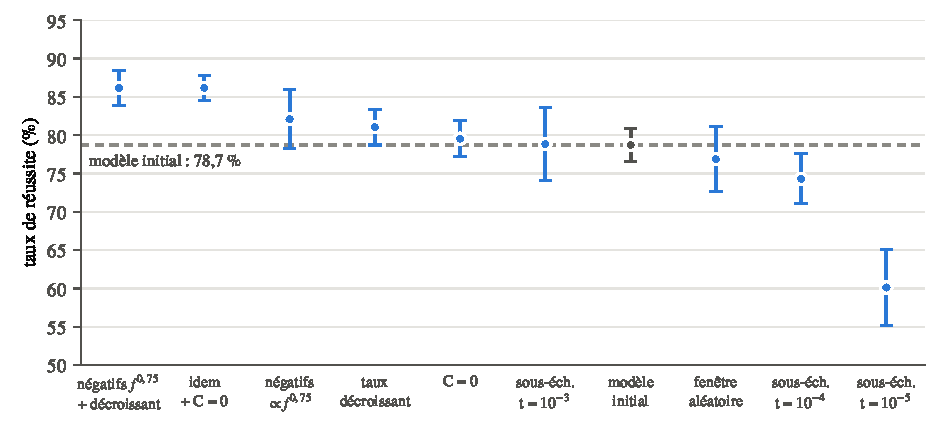
\includegraphics[width=0.88\linewidth]{figures/figure1.pdf}
\caption{taux de réussite moyen et écart-type pour chaque configuration (10 graines). La ligne horizontale indique la moyenne du modèle initial.}
\end{figure}

\textbf{Les deux modifications validées~: H1 et H3.} Tirer les négatifs selon fréquence\textasciicircum{}0,75 fait gagner 3,4 points, et le taux décroissant 2,3 points. Chacune est significative au seuil de 5~\% (p ≈ 0,03). Un détail renforce ces résultats~: aucune des deux ne fait jamais moins bien que le modèle initial avec la même graine.

\textbf{Leur combinaison.} La configuration qui cumule les deux atteint 86,2~\%, soit +7,4 points, ce qui dépasse la somme des gains obtenus séparément (3,4 + 2,3 = 5,7). Les deux effets se renforcent donc. Nous pouvons proposer une explication, qui reste une hypothèse que nous n’avons pas vérifiée~: avec des négatifs tirés selon la fréquence, les mots fréquents reçoivent beaucoup plus de mises à jour que les autres, et la diminution du taux d’apprentissage stabiliserait ces vecteurs fortement sollicités en fin d’entraînement.

\textbf{Le sous-échantillonnage (H2)~: hypothèse invalidée sur notre corpus.} Plus le seuil t est petit, plus le score baisse~: +0,1 point pour t = 10⁻³ (aucune différence), -4,4 points pour 10⁻⁴, -18,6 points pour 10⁻⁵. Le corpus, déjà petit, perd l’essentiel de son information. Cela correspond à l’usage prévu par l’article, qui vise l’accélération de l’entraînement sur des corpus de plusieurs milliards de mots, où l’on peut se permettre de jeter beaucoup d’occurrences sans perte de qualité.

\textbf{La fenêtre aléatoire (H4)~: non validée.} La différence (-1,9 point, p = 0,24) n’est pas significative~: nous ne pouvons pas affirmer que la modification dégrade les résultats, seulement qu’elle ne les améliore pas.

\textbf{L’initialisation de C à zéro (H5)~: sans effet, comme attendu.} Le gain de 0,8 point n’est pas significatif (p = 0,43), et l’ajouter à la meilleure combinaison ne modifie pas la moyenne (86,2~\% dans les deux cas).

\subsection{Piste à creuser 2~: analogies et recherche du plus proche voisin}

\subsubsection{Description}

Si l’on prend les vecteurs de \emph{roi}, \emph{homme} et \emph{femme}, le calcul roi - homme + femme devrait donner un vecteur proche de celui de \emph{reine}. Le sujet demande de vérifier si cela est vrai sur un ensemble de 100 analogies de natures différentes, construit à la main, et d’utiliser pour cela des plongements appris sur un grand corpus.

Une analogie est un quadruplet (a, b, c, d), qui se lit «~a est à b ce que c est à d~». On calcule donc x = b - a + c, qui doit se trouver près du vecteur de d, puis on cherche dans le vocabulaire le mot dont le plongement est le plus proche de x, au sens de la distance euclidienne imposée par le sujet.

Les mots a, b et c sont exclus de la recherche. L’analogie est considérée comme réussie en top-1 si le mot attendu est le plus proche, et en top-5 s’il figure parmi les cinq plus proches.

Cette évaluation pose un problème algorithmique~: le vecteur x ne correspond à aucun mot, donc chaque analogie demande de chercher le plus proche voisin d’un point parmi N vecteurs de dimension n.

La méthode naïve compare x aux N vecteurs, ce qui coûte de l’ordre de N × n opérations par requête.

Le sujet cite les arbres k-d comme méthode plus efficace et demande de choisir un algorithme efficace parmi ceux de la littérature.

\textbf{H1~: l’arithmétique des vecteurs retrouve une part substantielle des analogies, avec de fortes différences selon le type de relation.} Les relations régulières et grammaticales devraient mieux réussir que les relations sémantiques plus floues.

\textbf{H2~: l’arbre k-d n’apporte aucun gain en dimension 100.} Un arbre k-d n’est efficace que si le nombre de points N est très grand devant 2\textasciicircum{}k, où k est la dimension (Friedman, Bentley et Finkel, 1977). Ici k = 100 et N = 2·10⁵, très loin de la condition.

\textbf{H3~: une méthode approchée est beaucoup plus rapide pour une perte de précision faible et réglable.}\nopagebreak

\textbf{Choix de l’algorithme approché.} Plusieurs familles de méthodes approchées existent~: le hachage sensible à la localité (LSH, Indyk et Motwani, 1998), la quantification de produit (Jégou, Douze et Schmid, 2011), les graphes de navigation comme HNSW.

Nous avons retenu l’index inversé par k-means (IVF) pour trois raisons~: il est simple et peut être programmé en entier à partir de la définition, il est couramment employé en grande dimension, et il n’a qu’un seul paramètre de réglage, nprobe, qui permet de tracer directement la courbe temps / précision demandée par H3.

On partitionne le vocabulaire en groupes par un algorithme des k-means. Chaque groupe est représenté par son centre. Pour une requête, on calcule d’abord la distance de x aux centres, on retient les nprobe groupes dont le centre est le plus proche, et on ne compare x qu’aux mots de ces groupes. La recherche est donc approchée~: le vrai plus proche voisin peut se trouver dans un groupe qu’on ne visite pas. Plus nprobe est grand, plus on a de chances de le trouver, et si on visite tous les groupes on retombe sur la recherche exacte.

Cette méthode suppose que les données forment des amas, ce qui est le cas des plongements de mots, dont les voisins sont regroupés par thèmes. Nous avons aussi programmé l’arbre k-d, d’une part parce que le sujet le mentionne, d’autre part pour pouvoir tester H2 par la mesure plutôt que par le seul raisonnement.

\subsubsection{Mise en œuvre}

\textbf{Modèle de plongements.}\nopagebreak

Nos propres plongements (6~759 mots) sont trop peu nombreux pour que la question algorithmique ait un sens, et appris sur un corpus trop petit pour contenir les mots d’analogies courantes comme les capitales.

Comme le suggère le sujet, nous avons utilisé le modèle d’identifiant 43 du dépôt de modèles NLPL (Fares, Kutuzov, Oepen et Velldal, 2017). C’est un modèle pour le français, appris avec l’algorithme Word2Vec Continuous Skipgram sur le corpus French CoNLL17, avec une fenêtre de 10 mots, des vecteurs de dimension 100 et un vocabulaire de 2~567~698 mots, sans lemmatisation.

Nous l’avons limité à ses 200~000 premiers mots, la même restriction pour toutes les méthodes comparées.

\textbf{Jeu d’analogies.}\nopagebreak

Nous avons construit à la main 100 analogies réparties en dix catégories (Tableau 7), parmi lesquelles les quatre exemples donnés par le sujet. Trois analogies sont ignorées parce qu’un de leurs mots est absent des 200~000 mots retenus (\emph{mangeai}, \emph{chanterais} et \emph{oison}), ce qui laisse \textbf{97 analogies évaluées}~: tous les taux de cette section sont calculés sur 97.

Trois méthodes ont été explorées~:

\textbf{Recherche naïve.} Calcul de la distance de x à tous les mots, en une seule opération matricielle.

\textbf{Arbre k-d.} L’arbre est construit récursivement~: à chaque nœud, on sépare les points selon la dimension dans laquelle ils sont les plus dispersés (variance maximale), en coupant à la médiane, jusqu’à obtenir des feuilles d’environ 20 mots.

La recherche descend vers la feuille de x, puis remonte en abandonnant toute branche dont la distance au plan de coupe dépasse déjà la meilleure distance trouvée.

Nous avons ajouté au code un compteur de mots effectivement comparés, pour mesurer directement l’efficacité de l’élagage.

\textbf{IVF.} Le nombre de groupes est la racine carrée du nombre de mots, soit 447, l’algorithme est entraîné sur un échantillon de 50~000 mots, avec 10 itérations, pour que la construction reste courte. Nous testons nprobe = 1, 5, 10, 20 et 50.

\textbf{Contrôle de validité.}\nopagebreak

La méthode naïve fournit la référence exacte, et nous comptons, pour chaque autre méthode, le nombre d’analogies dont la réponse (le mot le plus proche) est identique à celle de la méthode naïve.

\textbf{Difficultés rencontrées.} Nos premières mesures de temps avaient été faussées par des calculs lancés en même temps sur la machine, elles ont été refaites une méthode à la fois.

\subsubsection{Résultats}

\begin{table}[!htbp]
\centering
\small
\caption{temps et précision des méthodes de recherche sur 97 analogies et 200~000 mots. La dernière colonne compte les analogies dont la réponse est identique à celle de la méthode naïve.}
\begin{tabular}{lccccc}
\toprule
\textbf{méthode} & \textbf{construction} & \textbf{recherche par analogie} & \textbf{top-1} & \textbf{top-5} & \textbf{identiques à la naïve} \\
\midrule
naïve & 0 s & 30,3 ms & 67,0~\% & 79,4~\% & – \\
arbre k-d & 0,86 s & 150,6 ms & 67,0~\% & 79,4~\% & 97 / 97 \\
IVF, nprobe = 1 & 1,25 s & 0,2 ms & 46,4~\% & 51,5~\% & 60 / 97 \\
IVF, nprobe = 5 & 1,26 s & 0,8 ms & 64,9~\% & 76,3~\% & 92 / 97 \\
IVF, nprobe = 10 & 1,24 s & 1,7 ms & 66,0~\% & 78,4~\% & 93 / 97 \\
IVF, nprobe = 20 & 1,24 s & 3,7 ms & 66,0~\% & 78,4~\% & 95 / 97 \\
IVF, nprobe = 50 & 1,23 s & 9,5 ms & 67,0~\% & 79,4~\% & 97 / 97 \\
\bottomrule
\end{tabular}
\end{table}

\begin{figure}[!htbp]
\centering
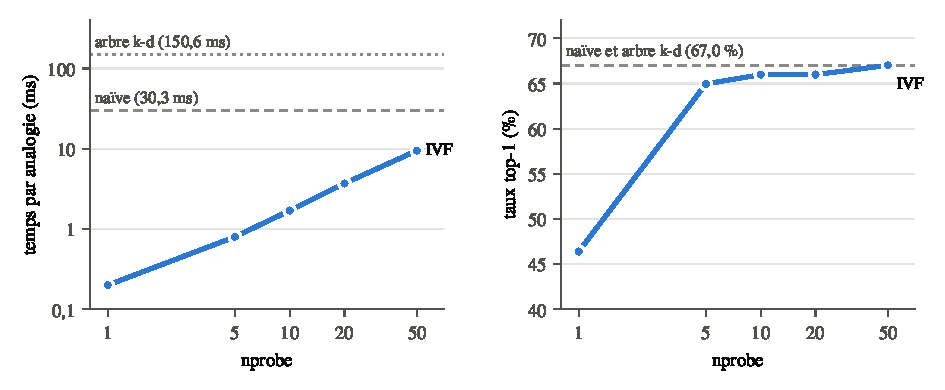
\includegraphics[width=0.88\linewidth]{figures/figure2.pdf}
\caption{temps de recherche par analogie et taux top-1 de l’IVF en fonction de nprobe (échelle logarithmique en abscisse, et en ordonnée pour les temps). Les lignes horizontales donnent les valeurs de la méthode naïve et de l’arbre k-d.}
\end{figure}

\begin{table}[!htbp]
\centering
\small
\caption{taux de réussite top-1 par catégorie, avec la méthode exacte (65 réussites sur 97).}
\begin{tabular}{llc}
\toprule
\textbf{catégorie} & \textbf{exemple (a, b, c, d)} & \textbf{top-1} \\
\midrule
pays → nationalité & France, français, Allemagne, allemand & 9 / 10 \\
pluriel & cheval, chevaux, animal, animaux & 9 / 10 \\
genre & homme, femme, roi, reine & 11 / 15 \\
pays → capitale & Allemagne, Berlin, Italie, Rome & 10 / 15 \\
conjugaison & mangeons, mangez, chantons, chantez & 9 / 14 \\
dérivation (adverbe, comparatif, nom) & heureux, heureusement, lent, lentement & 4 / 5 \\
suites, saisons et fleuves & un, deux, trois, quatre & 4 / 6 \\
contraires & grand, petit, long, court & 2 / 4 \\
arbre → fruit & cerisier, cerise, bananier, banane & 1 / 4 \\
petit de l’animal & chien, chiot, chat, chaton & 2 / 3 \\
exemples du sujet & pommier, pomme, poirier, poire & 1 / 3 \\
métier → lieu ou objet & médecin, hôpital, professeur, école & 3 / 8 \\
\bottomrule
\end{tabular}
\end{table}

\textbf{H1~: validée, avec de fortes différences selon les relations.}\nopagebreak

La méthode exacte retrouve 67,0~\% des analogies en top-1 et 79,4~\% en top-5~: l’arithmétique des vecteurs fonctionne dans une bonne partie des cas.

Les relations régulières et morphologiques réussissent le mieux (nationalités 9/10, pluriels 9/10, conjugaisons 9/14), les relations sémantiques indirectes beaucoup moins (métier → lieu 3/8, arbre → fruit 1/4).

Mais plusieurs catégories ne contiennent que 3 à 6 analogies, et un écart d’une analogie y change le taux de 20 à 30 points. L’écart entre top-1 et top-5 (12 analogies) montre que l’erreur est souvent un quasi-succès~: le modèle a trouvé la bonne catégorie mais pas le bon élément.

C’est le cas le plus fréquent. On le retrouve en conjugaison~: pour \emph{sais, savons, peux, ?}, le modèle propose \emph{voulons}, \emph{aimerions}, \emph{devons}, puis seulement \emph{pouvons}~: il a identifié la forme (première personne du pluriel) et le champ (verbes modaux), mais pas le verbe.

Un plongement statique n’a qu’un vecteur par forme, donc tous les sens du mot sont confondus. Pour \emph{oranger, orange, citronnier, ?}, le modèle répond \emph{mobile}, \emph{wildfire}, \emph{rim}~: le vecteur de \emph{orange} semble dominé par l’opérateur de téléphonie, ce qui reste à confirmer.

Le même phénomène touche \emph{chienne}, employé surtout dans un sens injurieux dans un corpus issu du web.

C’est une limite structurelle des plongements statiques, que les plongements contextuels cherchent à lever.

\emph{Orthographe et bruit du modèle.} Le vocabulaire du modèle, issu de textes du web, contient des variantes (\emph{hanoi} et \emph{hanoï}, \emph{soeur} et \emph{sœur}, \emph{patisserie} et \emph{pâtisserie}) et des formes mal segmentées avec leur ponctuation (\emph{jour!}, \emph{jour?}, \emph{,vous}, \emph{...soit}, \emph{printemps!}). Cela montre que la qualité du prétraitement du modèle externe affecte le score indépendamment de la méthode.

\textbf{Portée de ces résultats.}\nopagebreak

Les taux dépendent à la fois du modèle (appris sur un très gros corpus, avec une fenêtre de 10) et de notre jeu d’analogies (mots courants, relations choisies par nous). Ils ne sont pas comparables à ceux d’autres jeux, ni à ceux qu’on obtiendrait avec nos plongements de la section 2. Il a d’ailleurs été intéressant de voir que les camarades ayant travaillé sur le même sujet avaient des taux bien différents.

\textbf{H2~: validée, et mesurée directement.}\nopagebreak

L’arbre k-d fournit exactement les mêmes réponses que la méthode naïve pour les 97 analogies, ce qui confirme qu’il est exact et correctement implémenté.

Mais le compteur placé dans la recherche indique que \textbf{100~\% des mots sont examinés} à chaque requête~: l’élagage n’écarte jamais aucune branche, exactement comme le prévoit le raisonnement sur la grande dimension (2\textasciicircum{}100 est de l’ordre de 10³⁰, très au-delà de N = 2·10⁵).

L’arbre est donc, en plus, cinq fois plus lent que le parcours naïf (150,6 ms contre 30,3 ms)~: il fait le même nombre de comparaisons, mais en plus de la descente dans l’arbre. Ce facteur 5 dépend aussi de notre implémentation (arbre écrit en Python, recherche naïve faite en un seul calcul matriciel), alors que les 100~\% de mots examinés n’en dépendent pas.

\textbf{H3~: validée, avec un compromis chiffré.}\nopagebreak

\begin{itemize}

\item Pour nprobe = 10, la recherche est environ 18 fois plus rapide que la méthode naïve (1,7 ms contre 30,3 ms), pour une seule analogie réussie en moins (66,0~\% contre 67,0~\%), seules 4 réponses sur 97 diffèrent de celles de la méthode exacte.

\item Pour nprobe = 50, les 97 réponses sont identiques à celles de la méthode exacte, et la recherche reste environ 3 fois plus rapide.

\item Pour nprobe = 1, la précision s’effondre (46,4~\%)~: pour 37 analogies sur 97, la réponse n’est pas celle de la méthode exacte. Le mot le plus proche de x se trouve donc fréquemment dans un autre groupe que celui dont le centre est le plus proche.

\item La construction de l’index coûte 1,24 s et fait gagner environ 28,6 ms par requête~: elle est amortie au bout d’une quarantaine de requêtes (1,24 / 0,0286 ≈ 43). Pour 97 analogies, le gain est net. Pour une requête isolée, la méthode naïve reste préférable.

\end{itemize}

\section{Conclusions et perspectives}

\subsection{Bilan}

Ce projet avait pour objectif de programmer un modèle de plongements de mots statiques de type skip-gram avec échantillonnage négatif, puis d’explorer deux pistes~: améliorer ses performances (piste 1), et vérifier la capacité des plongements à retrouver des analogies en cherchant efficacement le mot le plus proche d’un vecteur (piste 2).

Le Tableau 8 rappelle le résultat de chaque hypothèse formulée.

\begin{table}[!htbp]
\centering
\small
\caption{bilan des hypothèses.}
\begin{tabularx}{\linewidth}{c>{\raggedright\arraybackslash}X>{\raggedright\arraybackslash}X}
\toprule
\textbf{piste} & \textbf{hypothèse} & \textbf{verdict} \\
\midrule
1 & H1~: négatifs tirés selon fréquence\textasciicircum{}0,75 & validée (+3,4 points) \\
1 & H2~: sous-échantillonnage des mots fréquents & invalidée sur notre corpus (de 0 à -18,6 points selon t) \\
1 & H3~: taux d’apprentissage décroissant & validée (+2,3 points) \\
1 & H4~: fenêtre de taille aléatoire & non validée (-1,9 point, non significatif) \\
1 & H5~: matrice C initialisée à zéro & sans effet, comme attendu \\
2 & H1~: l’arithmétique des vecteurs retrouve des analogies, selon le type de relation & validée (67,0~\% en top-1) \\
2 & H2~: l’arbre k-d n’apporte aucun gain en dimension 100 & validée (100~\% des mots examinés, 5 fois plus lent) \\
2 & H3~: une méthode approchée (IVF) est bien plus rapide pour une faible perte de précision & validée (18 fois plus rapide pour une analogie réussie en moins) \\
\bottomrule
\end{tabularx}
\end{table}

Deux modifications simples améliorent nettement le modèle. Tirer les négatifs selon fréquence\textasciicircum{}0,75 et diminuer linéairement le taux d’apprentissage font passer le taux de réussite de 78,7~\% à 86,2~\%, sans toucher à la structure du modèle. La première modification vient de l’article, la seconde seulement du code officiel, ce qui montre qu’un article ne décrit pas tout ce que fait l’implémentation de référence.

Le sous-échantillonnage, présenté par l’article comme une amélioration, dégrade nos résultats, de plus en plus quand le seuil t diminue. En revanche, le gain de temps annoncé par l’article est bien observé (environ 17 secondes d’entraînement au lieu de 150).

La structure de données suggérée par le sujet ne convient pas ici, et une méthode approchée est préférable. L’arbre k-d donne les mêmes réponses que la recherche exhaustive, mais il compare 100~\% des mots à chaque requête~: en dimension 100, son élagage n’écarte aucune branche, comme le laisse prévoir la théorie. L’index inversé IVF est, avec nprobe = 10, environ 18 fois plus rapide que la recherche exhaustive pour une seule analogie réussie en moins sur 97, et avec nprobe = 50 il donne exactement les mêmes réponses tout en restant 3 fois plus rapide.

Sur le fond, les analogies fonctionnent dans une bonne partie des cas (67,0~\% en top-1, 79,4~\% en top-5), surtout pour les relations régulières comme les pluriels, les conjugaisons et les nationalités, et beaucoup moins pour les relations sémantiques indirectes. Les erreurs que nous avons relevées s’expliquent en grande partie par une limite connue des plongements statiques~: un seul vecteur par mot, donc tous les sens d’un mot polysémique confondus.

\subsection{Limites}

\begin{itemize}

\item \textbf{Le corpus et le jeu d’évaluation ne sont pas ceux du sujet.} Nous avons travaillé sur un corpus de substitution et seuls 86 triplets sur 100 sont évaluables. Avec 86 triplets, un triplet change le taux d’environ 1,2 point~: la résolution de la mesure est grossière, et les écarts inférieurs à 2 ou 3 points sont difficiles à interpréter.

\item \textbf{Les explications avancées sont des hypothèses.} Nous n’avons pas vérifié le mécanisme qui explique pourquoi les deux modifications retenues se renforcent, ni la cause exacte de certaines erreurs d’analogies.

\end{itemize}

\subsection{Perspectives}

Piste 1.

\begin{itemize}

\item Refaire la comparaison sur un corpus beaucoup plus grand (plusieurs dizaines de millions de mots), pour tester si c’est bien la taille du corpus qui invalide l’hypothèse sur le sous-échantillonnage, et chercher à partir de quel seuil t son effet devient favorable.

\item Retester la fenêtre aléatoire avec une demi-fenêtre plus grande (par exemple L = 5, valeur du code officiel), car avec L = 2 la modification retire environ un quart des paires.

\item Faire varier le nombre de négatifs k et la dimension n, que nous avons laissés aux valeurs du sujet.

\item Évaluer sur un jeu de triplets plus grand et adapté au corpus, pour réduire la résolution grossière de la mesure.

\end{itemize}

Piste 2.

\begin{itemize}

\item Comparer la distance euclidienne, imposée par le sujet, au cosinus, ou normaliser les vecteurs avant l’indexation. La géométrie des groupes du k-means change, ainsi sans doute que le meilleur réglage de nprobe.

\item Indexer le vocabulaire complet (2,5 millions de mots) pour voir si le gain de l’IVF augmente avec la taille du vocabulaire.

\item Augmenter le nombre d’analogies par catégorie, pour que les taux par catégorie deviennent interprétables.

\item Comparer l’IVF à d’autres méthodes approchées, comme HNSW ou LSH, qui sont largement utilisées en pratique.

\end{itemize}

\textbf{Pour relier les deux pistes.}\nopagebreak

Nos plongements (6~759 mots) et le modèle externe n’ont pas été évalués sur la même tâche. Évaluer les nôtres sur des analogies construites avec leur propre vocabulaire, et mesurer l’effet des améliorations de la piste 1 sur ce critère, permettrait de relier les deux parties.

\end{document}
